\subsection{Case03 - Echo server}
\label{P4_ether_case03}


En este caso de uso desarrollaremos un servidor de Echo que responda todos los pings que le lleguen. Como tal el programa P4 no es suficiente para probar esta funcionalidad, como ya se mencionó, se requiere de una plataforma que sea capaz de soportar el lenguaje P4, el \gls{bmv2}. \\
\par

El programa P4 deberá ser capaz de analizar los paquetes que le lleguen, analizarlos y filtrarlos. Solo aquellos paquetes filtrados serán los que se deberán responder. ¿Cómo se filtrarán? Se añadirán nuevos estados en el parser que comprueben si las cabeceras ICMP están presentes. Por ello, antes de nada se debe declarar las cabeceras ICMP necesarias para poder así analizar las cabeceras de los paquetes que lleguen.

\begin{lstlisting}[language=C, style=P4-color, caption={Estructura cabecera ICMP - Case03},label=code:case03_p4_ether_prog1]
    header icmp_t {
    	bit<8> type;
    	bit<8> code;
    	bit<16> checksum;
    }
\end{lstlisting}
\vspace{0.5cm}

Como se quería que este programa P4 fuera compatible con direccionamiento IPv6 se han añadido también los equivalentes en ICMPv6 y la cabecera de red de IPv6, ver bloque \ref{code:case03_p4_ether_prog2}.

\begin{lstlisting}[language=C, style=P4-color, caption={Estructura cabeceras IPv6 e ICMPv6  - Case03},label=code:case03_p4_ether_prog2]
    header ipv6_t {
       bit<4> version;
       bit<8> trafficClass;
       bit<20> flowLabel;
       bit<16> payloadLen;
       bit<8> nextHdr;
       bit<8> hopLimit;
       ip6Addr_t srcAddr;
       ip6Addr_t dstAddr;	
    }
    
    
    header icmp6_t {
       bit<8> type;
       bit<8> code;
       bit<16> checksum;
    }
\end{lstlisting}
\vspace{0.5cm}

Ahora que ya se tiene las cabeceras definidas, se deberá preocuparse en definir las macros asociadas a los posibles \textit{ethertypes} que se quieran manejar, IPv4 y IPv6. De forma adicional, se deberán definir los códigos de protocolo de las cabeceras de red, para asegurare que sobre la cabecera de red únicamente se procesarán aquellos paquetes que porten información ICMP. Se tuvo que consultar la RFC asociada a IPv6 para saber que codificación hacían con el campo de \textit{nextHeader} y por lo visto utilizan los mismo valores que en IPv4. A continuación, en la figura \ref{code:case03_p4_ether_prog3} se puede ver la definición de dichas macros y el extracto de la RFC asociada a la codificación de las cabeceras IPv6 .\\
\par

\begin{lstlisting}[language=C, style=P4-color, caption={Macros para parsear L2 y L3  - Case03},label=code:case03_p4_ether_prog3]
    /*	---	Layer 2 MACROS	     ---	*/
    const bit<16> ETHERTYPE_IPV4 = 0x0800;
    const bit<16> ETHERTYPE_IPV6 = 0x86dd;
    
    /*	---	Layer 3 MACROS	     ---	*/
    const bit<8> IP_PROTOCOL_ICMP = 0x01;
    const bit<8> IP_PROTOCOL_ICMPv6 = 0x3a; 
    const bit<8> ICMP_ECHO_REQUEST_TYPE = 0x08;
    const bit<8> ICMP_ECHO_REQUEST_CODE = 0x00;
    const bit<8> ICMP_ECHO_REPLY_TYPE = 0x00;
    const bit<8> ICMP_ECHO_REPLY_CODE = 0x00;
    
    /*
    *   According to RFC 2460, the codes of the protocol immediately above,
    *   layer 4, are the same as those used in IPv4. And I quote:
    *
    *   Next Header          8-bit selector.  Identifies the type of header
    *                       immediately following the IPv6 header.  Uses the
    *                       same values as the IPv4 Protocol field [RFC-1700
    *                       et seq.].
    *
    */
\end{lstlisting}
\vspace{0.5cm}

Como se ha indicado en el bloque \ref{code:case03_p4_ether_prog3},  de forma adicional se han definido macros sobre los valores con los que se va estar trabajando (\texttt{ECHO-Request} y \texttt{ECHO-Reply}). De esta forma el código resultante de las \textit{actions} será más interpretable y sostenible. Teniendo ya todas las herramientas necesarias para declarar los nuevos estados del parser, se puede proceder con el siguiente bloque del datapath.\\
\par

Una vez que se es capaz de filtrar los paquetes que interesan, se va a ver cómo se ha implementado la lógica de procesamiento de aquellos paquetes que ya han sido filtrados. Es de interés interceptar todos los paquetes ICMP que lleguen a nuestro ``switch" para así contestarlos desde el mismo "switch". Por ello, se hará uso del bit de validez de las cabeceras que han sido analizadas correctamente, es decir, si el paquete contiene dichas cabeceras. De no contenerlas, su bit de validez estará a \textit{false}. A continuación en la figura \ref{code:case03_P4_ether_prog4}, mostramos la lógica de control del bloque \textit{Ingress}.


\begin{lstlisting}[language=C, style=P4-color, caption={Lógica para filtrar paquetes ICMP e ICMPv6  - Case03},label=code:case03_P4_ether_prog4]
    /*  
     *  De esta forma nos aseguramos que unicamente procesamos paquetes ICMP,
     *  o en su defecto ICMPv6.
     *
     */
    
    
    apply {
    	if(hdr.ipv4.isValid() && hdr.icmp.isValid()){
    	        echo();
    	}else if (hdr.ipv6.isValid() && hdr.icmp6.isValid()){
    		echo6();
    	}
    }
\end{lstlisting}
\vspace{0.5cm}

Ya se tienen todos los paquetes ICMP filtrados, solo quedaría programar la lógica para modificar las cabeceras de dicho paquete para conseguir contestar satisfactoriamente al emisor del ping. Para ello, se hará uso de un \textit{action}, una función. El cual intercambiará tanto MAC destino-origen, como IP destino-origen, modificará la cabecera ICMP para indicarle que se trata de un \textit{reply}, y por último mandará el paquete por el puerto por el cual llegó al \gls{bmv2}, de esta forma se asegura que dicho paquete llegará al emisor del mismo.\\
\par


\begin{lstlisting}[language=C, style=P4-color, caption={Lógica para procesar paquetes ICMP  - Case03},label=code:case03_p4_ether_prog5]
    action echo (){
    	/*	---	Auxiliary variables	---	*/
        macAddr_t temp_mac = hdr.ethernet.srcAddr;
        ip4Addr_t temp_ip = hdr.ipv4.srcAddr;
    
    	/*      ---     Swap MACs     ---     */
    	hdr.ethernet.srcAddr = hdr.ethernet.dstAddr;
        hdr.ethernet.dstAddr = temp_mac;
    
    	/*      ---     Swap Ips     ---     */
     	hdr.ipv4.srcAddr = hdr.ipv4.dstAddr;
    	hdr.ipv4.dstAddr = temp_ip;
      
    	/*      ---     Re-Write ICMP's type and code     ---     */
    	hdr.icmp.type = ICMP_ECHO_REPLY_TYPE;
    	hdr.icmp.code = ICMP_ECHO_REPLY_CODE;
    
    	/*      ---     Forward the packet to the ingress intf     ---     */
    	standard_metadata.egress_spec = standard_metadata.ingress_port;

    }  
\end{lstlisting}
\vspace{0.5cm}

\newpage

Préstese atención a la última sentencia de la función donde le indicamos que saque el paquete por la misma interfaz por la cual ha entrado. Este es el equivalente directo al código de retorno en \gls{xdp}, \texttt{XDP\_TX} con el cual re-circulábamos el paquete de la misma forma a la interfaz de entrada.\\
\par

Como curiosidad, es interesante comentar que el campo \textit{checksum} de la cabecera ICMP debe ser re-calculado de nuevo por lo que se deberá hacer antes del \textit{Egress}. Esto supuso un problema, ya que continuamente estaban saliendo paquetes con un \textit{checksum} incorrecto,  lo cual se comprobó con el disector de Wireshark. Finalmente se vio que no había que incluir el campo \textit{checksum} en la nueva suma del nuevo \textit{checksum}\footnote{Habría sido genial que la RFC asociada hubiera estado más clara al respecto.}, de esta forma los paquetes \texttt{ECHO-Reply} que salían ya llevaban el \textit{checksum} calculado correctamente.\\
\par


\vspace{1cm}
\textbf{Compilación y puesta en marcha del escenario}\\
\par

Para la compilación del programa P4 se hará uso de nuevo del compilador P4c (más información sobre el proceso de compilación en la subsección \ref{p4_ether_case01}).\\
\par

Dado que las personas que quieran replicar los casos de uso puede que no estén muy familiarizadas con todo este proceso de compilación y carga en los procesos de \gls{bmv2}, se ha dispuesto un de un Makefile para automatizar las tareas de compilación y carga, y las tareas de limpieza del caso de uso. Para la puesta en marcha del caso de uso se deben seguir los pasos indicados en el bloque \ref{code:case03_p4_ether_load}.\\
\par

\begin{lstlisting}[language= bash, style=Consola, caption={Compilación programa P4 y puesta en marcha del escenario - Case03},label=code:case03_p4_ether_load]
    # Entramos al directorio 
    cd TFG/src/use_cases/p4/case03

    # Hacemos uso del Makefile
    sudo make run
\end{lstlisting}
\vspace{0.5cm}

Una vez se haya finalizado la comprobación del funcionamiento del caso de uso, se debe hacer uso de otro target (\textit{clean}) del Makefile para limpieza total del directorio según se indica en el bloque \ref{code:case03_p4_ether_unload}.

\begin{lstlisting}[language= bash, style=Consola, caption={Limpieza del escenario P4 - Case03},label=code:case03_p4_ether_unload]
    # Hacemos uso del Makefile
    sudo make clean
\end{lstlisting}
\vspace{0.5cm}

Es importante señalar que este target limpiará tanto los ficheros auxiliares para la carga del programa P4 en el \gls{bmv2}, como los directorios de \texttt{pcaps}, \texttt{log}, y \texttt{build} generados en la puesta en marcha del escenario. Por lo que si se desea conservar las capturas de las distintas interfaces de los distintos \gls{bmv2}, se deben copiar o limpiar del escenario a mano siguiendo las indicaciones del bloque \ref{code:case03_p4_ether_unload2}.\\
\par

\begin{lstlisting}[language= bash, style=Consola, caption={Limpieza segura del escenario P4 - Case03},label=code:case03_p4_ether_unload2]
    # Limpiamos Mininet
    sudo mn -c
    
    # Limpiamos los directorios generados dinámicamente en la carga del escenario
    sudo rm -rf build logs
\end{lstlisting}


\vspace{1cm}
\textbf{Comprobación del funcionamiento}\\
\par

Una vez realizado el make run en este directorio, se tendrá levantada la topología descrita para este caso de uso, la cual se puede apreciar en la figura \ref{fig:case03_p4_ether_scenario}. Como en el \textit{datapath} no se contempla el manejo del protocolo ARP, se ha añadido el ARP entry a directamente en los hosts, desde el fichero \texttt{topology.json} consiguiendo así que no se genere la resolución ARP en el envío de los \texttt{ECHO-Request}. En este caso, la demostración se va hacer uso de IPv4, en el caso de querer hacerla con IPv6, se deberá añadir la entrada analoga para el protocolo ND  (\textit{Neighbor Discovery}).\\
\par
% figura escenario
\begin{figure}[ht]
    \centering
    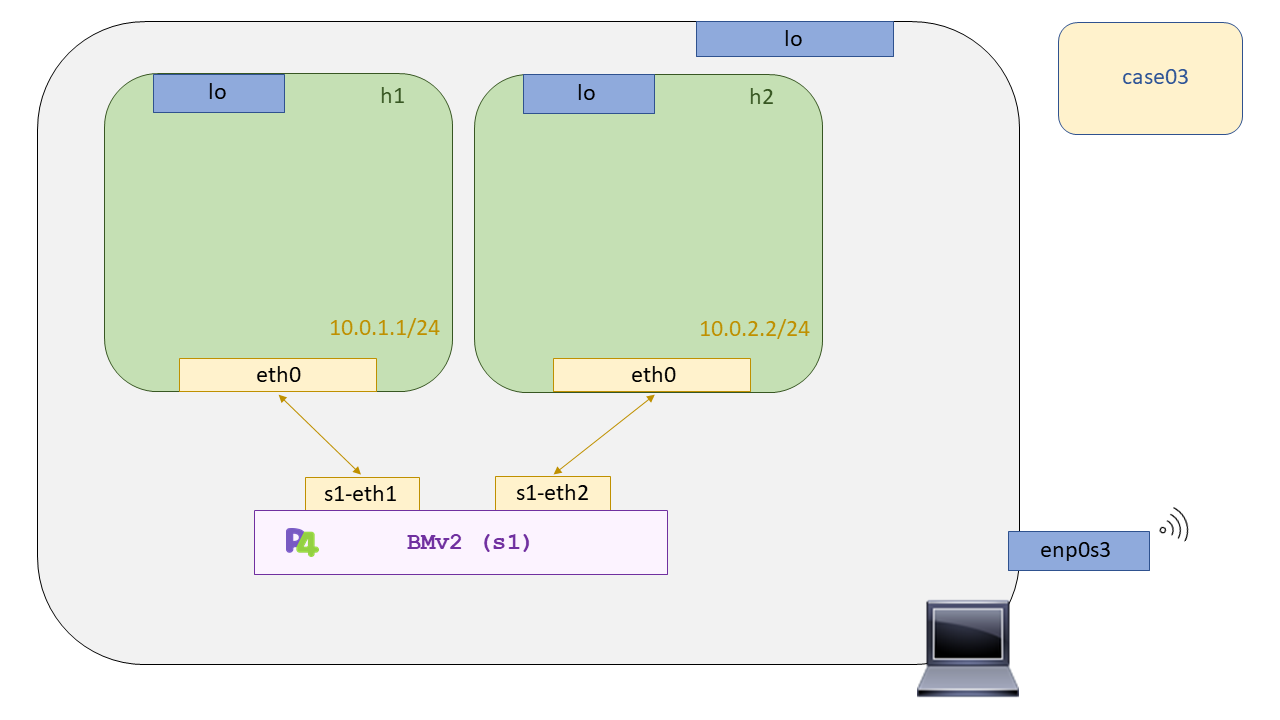
\includegraphics[width=16cm]{archivos/img/dev/p4/case03/scenario.png}
    \caption{Escenario del Case03 - P4}
    \label{fig:case03_p4_ether_scenario}
\end{figure}

Volviendo de nuevo a la comprobación del funcionamiento del caso de uso, se tendrá la CLI de Mininet abierta, por lo que se procederá a abrir una terminal para el \texttt{host1}, desde el cual se llevará a cabo los pings.

\begin{lstlisting}[language= bash, style=Consola, caption={Comprobación de funcionamiento - Case03},label=code:case03_p4_ether_func]
    mininet>  xterm h1
\end{lstlisting}
\vspace{0.5cm}

Una vez que se tenga la terminal abierta, se procederá a abrir Wireshark. En este caso se recomineda Wireshark ya que se podrá filtrar y comprobar de una forma más sencilla la validez de los \textit{checksums}.

% figura escenario
\begin{figure}[ht]
    \centering
    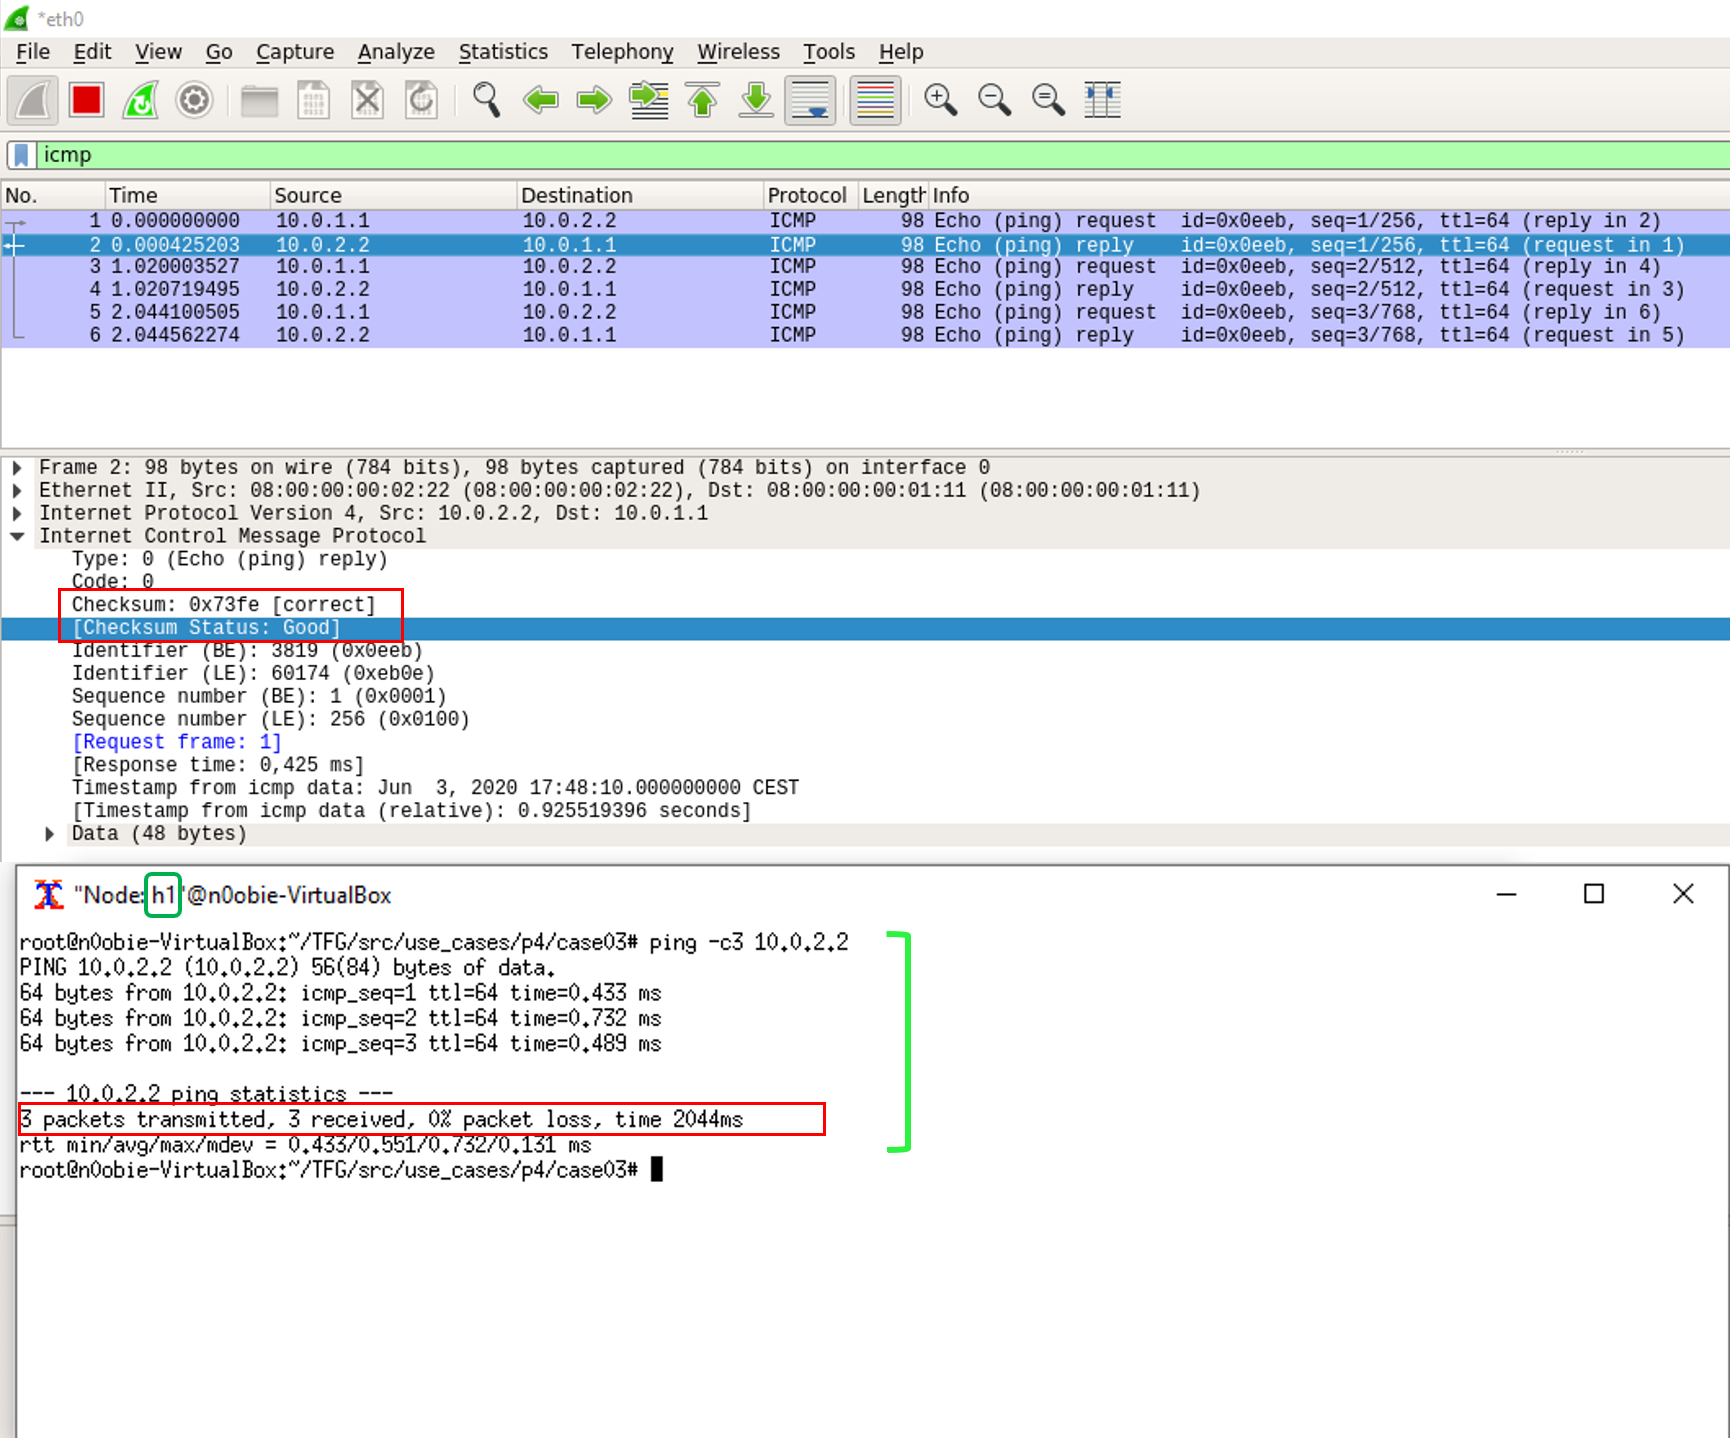
\includegraphics[width=15.5cm]{archivos/img/dev/p4/case03/demo_case03_edited.png}
    \caption{Comprobación de funcionamiento del Case03 - P4}
    \label{fig:case03_p4_ether_func1}
\end{figure}

Como se puede ver en la figura \ref{fig:case03_p4_ether_func1}, todo funciona correctamente ya que se están recibiendo respuesta a los pings \fcolorbox{black}{green}{\rule{0pt}{2.5pt}\rule{2.5pt}{0pt}}\hspace{1mm}. De forma adicional, se puede comprobar con Wireshark como el \textit{checksum} de la cabecera ICMP viene correctamente calculado.

